\documentclass[11pt,letterpaper]{article}
\usepackage[utf8]{inputenc}
\usepackage[margin=1in]{geometry}
\usepackage[margin=1cm]{caption}
\usepackage{amsmath}
\usepackage{amsfonts}
\usepackage{amssymb}
\usepackage{amsthm}
\usepackage{verbatim}
\usepackage{graphicx}
% No paragraph tabs
\setlength{\parindent}{0pt}

% Define commands that will be widely used.
\newcommand{\br}{\ \\}
\newcommand{\tab}{\hspace*{2em}}

\title{Atomic Physics Experiments}
\author{Rachel Domagalski\\
Partner: Matthew Turner}
\date{November 18, 2013}

\begin{document}
\maketitle

\begin{abstract}
    Atomic physics experiments serve as tests which can measure important
    physical constants. This lab presents two classic atomic physics
    experiments, in which the Rydberg constant and the Bohr magneton are
    measured. The experiment that measures the Rydberg constant is done through
    measuring the Balmer series spectral lines. The Bohr magneton is measured
    from Zeeman splitting. The value of the Rydberg constant determined from
    fitting to the Rydberg formula was measured to be
    $R = 1.095 \times 10^7 \pm 2 \times 10^4\ m^{-1}$. The measured value of the
    Bohr magneton was found to be
    $\mu_B = 1.49\times 10^{-23} \pm 2 \times 10^{-25}\ J/T$.
\end{abstract}

\section{Introduction}

Quantum mechanics has incredible importance in understanding the structure of
atoms. Therefore, atomic physics experiments serve as good experimental tests to
see if quantum mechanics is a valid theory, and studying spectral lines is
useful in testing quantum mechanics. Initially, when physicists first started
observing the spectrum of various elements, they discovered that the spectra did
not consist of continuous bands of color, but of sharp and discrete lines of
various colors. Classical physics did not provide any explanation for why this
happened. Quantum mechanics, however, was able to predict the wavelengths of the
spectral lines, as well as explain atomic interactions that gave rise to these
spectral lines.\\

In quantum mechanics, energy comes in discrete packets, called quanta. This is
different from classical mechanics where the energy distributions are
continuous. The standard interpretation of quantum mechanics is that a system
can be described by a wavefunction $\Psi$, which is a linear combination of the
eigenvectors of the system's Hamiltonian operator. Since the Hamiltonian is a
Hermitian operator, it's eigenvalues are observable quantities and the
eigenvalues of the Hamiltonian represent the energy of the system. In practice,
the energy levels are not directly measured, but the energy level differences
can be measured by measuring the wavelengths or frequencies of the light that
gets absorbed or emitted when a quantum system changes states. The spectra that
arises from the energy level changes can serve as a good probe of the quantum
system being measured.\\

Two areas of interest in atomic physics are the hydrogen and helium atoms.
Hydrogen is interesting because it is the only atom for which the
Schr\"{o}dinger equation can be solved analytically for the energy levels. It
should be noted that in the case of hydrogen, solving the  Schr\"{o}dinger
equation is not the only method to calculate the hydrogen energy levels. The
other method, which only works for hydrogen, is the Bohr model, but this model
is very limited. The energy levels of hydrogen will be measured in the lab and
will be used to calculate the Rydberg constant.\\

Helium is an interesting atom to study because it provides a simple two-level
system and experiments with Helium can be used to test perturbation theory. One
example of a system that requires perturbation theory to predict experimental
results is known as Zeeman splitting. Zeeman splitting is the effect which
occurs when electrons are placed in an external magnetic field. The reason that
it is called splitting is because energy levels which were degenerate without
the external field split and become non-degenerate when the field is applied.
When observed in the lab, this corresponds to a splitting of the spectral lines
of an atom. This effect can be used to measure the Bohr magneton.

\section{The Balmer Series}

The hydrogen atom can be approximated as point charge $e^-$ of mass $m$ in a
Coulomb potential from a positive charge $e$. The Schr\"{o}dinger equation for
that system is \cite{BransdenQM}
\begin{equation}
    \left[-\frac{\hbar^2}{2m}\nabla^2 - \frac{e^2}{4\pi \epsilon_0 r}\right]
        \psi = E\psi
    \label{sehydrogen}
\end{equation}

The eigenvalues for \eqref{sehydrogen} are \cite{BransdenQM}
\begin{equation}
    E_n = -\frac{m}{2\hbar^2}
        \left(\frac{e^2}{4\pi \epsilon_0}\right)^2
        \frac{1}{n^2}
        \approx -\frac{13.6\ eV}{n^2}
\end{equation}
When electrons transition from energy levels, they emit photons with energy 
$E = hc / \lambda$, which is equal to the difference between the energy levels
of the transition. Many different energy level transitions have been given
names, and the Balmer series is defined as transitions down to the $n = 2$
energy level. From this, it is easy to derive the Rydberg formula that gives the
Balmer lines.
\begin{equation}
    \frac{1}{\lambda_n} = R \left(\frac{1}{4} - \frac{1}{n^2}\right),
    \text{ where } R = \frac{m_e e^4}{8 \epsilon_0^2 h^3 c}
    \label{rydberg}
\end{equation}

The Balmer series is special because it is the only class of energy level
transitions for hydrogen that produces emission lines in the visible spectrum. 
The experiment involving hydrogen seeks to measure the Rydberg constant from
measuring the Balmer wavelengths. It can be seen from \eqref{rydberg} that the
Rydberg constant can be measured in two places, the slope and the intercept, 
from creating a linear fit of $1 / n^2$ and $1 / \lambda$.

\subsection{Experimental setup}

% Block diagram of the experiment
\begin{figure}
    \centering
    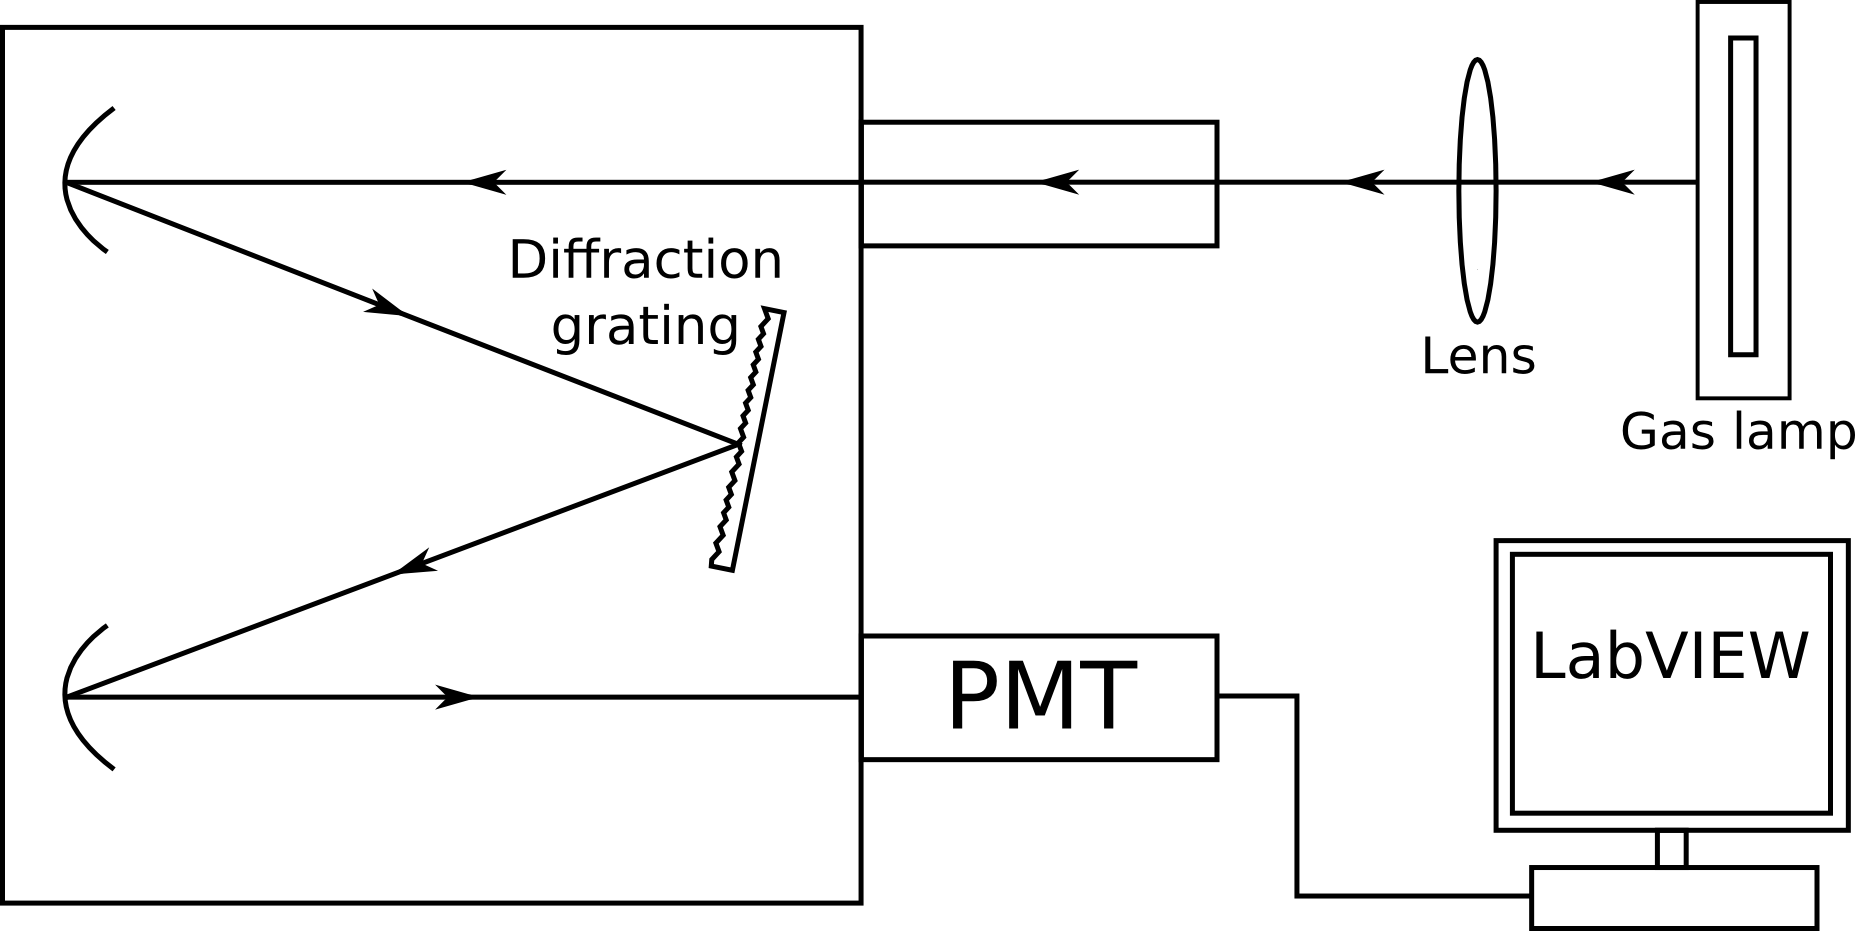
\includegraphics[width=0.6\textwidth]{figures/spectrometer.png}
    \caption{Block diagram of the spectrometer used to measure the Balmer
        lines.}
    \label{spectrometer}
\end{figure}

This experiment uses a spectrometer connected to a photomultiplier tube to
measure the emission lines of hydrogen (see Figure~\ref{spectrometer}). How this
works is that light from a hydrogen lamp gets focused into a spectrometer.
Inside the spectrometer are two mirrors and a diffraction grating, which are
used to reflect the light. The diffraction grating also has the function of
splitting the light which helps get better resolution on the wavelengths of
light. The light then moves on to the photomultiplier tube, which converts the
light into an electrical signal so it can be recorded. The data acquisition
process of the experiment is done with a digital multimeter that has a GPIB
output that gets fed into a computer running LabVIEW.\\

The experimental setup is pretty simple and straightforward. However, there are
some uncertainties in the measurements that must be accounted for. The first
uncertainty is the wavelength resolution of the spectrometer. The spectrometer
has a resolving power, which is defined as \cite{HechtOptics}
\begin{equation}
    R \equiv \frac{\lambda}{\Delta\lambda}
\end{equation}
In the case of diffraction gratings, the resolving power is \cite{HechtOptics}
\begin{equation}
    \frac{\lambda}{\Delta\lambda} = mN
\end{equation}
where $N$ is the number of grooves in the diffraction grating and $m$ is an
integer related to the propagation modes of the diffraction. For this
experiment, $m = 1$, and since the diffraction grating in the lab has 300
grooves per millimeter \cite{LabManual} and since the slit width of the
spectrometer can be adjusted from 0.005 $mm$ to 3 $mm$, the resolving power of
the grating is about 300.

\subsection{Line Broadening}

The second uncertainty in the wavelength comes from spectral line broadening.
While \eqref{rydberg} predicts sharp peaks in the spectrum at certain
wavelengths, very sharp distributions with nonzero widths are measured around
the absorption or emission peaks. This width in wavelength or frequency is what
is known as spectral line broadening. Spectral broadening has several causes,
three of which will be discussed, and the study of spectral line broadening has
useful applications in astrophysics. \\

The first mechanism of line broadening is called natural broadening. This
broadening comes from the Heisenberg uncertainty principle. The Heisenberg
uncertainty principle for time and energy states that
\begin{equation}
    \Delta E \Delta t \ge \frac{\hbar}{2}
\end{equation}

For a gas, the line profile that corresponds to natural broadening is
\cite{StellarAstro}
\begin{equation}
    \phi_\nu = \frac{\dfrac{\Gamma}{4\pi^2}}{\Delta\nu^2 + 
        \left(\dfrac{\Gamma}{4\pi}\right)^2}
    \label{lorentz}
\end{equation}
where $\Delta \nu = \nu - \nu_0$, and $\Gamma$ is the radiative damping
coefficient, which is just the reciprocal of the mean lifetime of a quantum
state, which is $\Delta t$ from the uncertainty principle. The mean lifetime is
on the order of $10\ ns$. The FWHM of \eqref{lorentz}, which corresponds to
$2\Delta \nu$ is equal to $\frac{\Gamma}{2\pi}$ \cite{StellarAstro}, which gives
the broadening in frequency space of 
\begin{equation}
    \Delta \nu = \frac{\Gamma}{4\pi} = \frac{1}{4\pi\Delta t}
    \label{natbrdnu}
\end{equation}

Since the experiment measures wavelengths and not frequencies, line broadening
values in frequency space will have to be converted to wavelength space. The
equation relating the frequency and wavelength of light waves $\lambda \nu = c$,
can be differentiated to get a relation for small spectral differences. This
gives $\nu d\lambda = -\lambda d\nu$ or 
$\nu \delta \lambda = \lambda \delta \nu$, where the signs of the differences
are neglected since line broadening occurs in both directions with respect to a
peak spectral line. From this, a relation between small wavelength shifts and
small frequency shifts can be found to be
\begin{equation}
    \delta \lambda = \frac{\lambda^2}{c} \delta \nu
    \label{broadswitch}
\end{equation}

The above relation can be used to get the natural line broadening width in
wavelength space. Plugging \eqref{natbrdnu} into \eqref{broadswitch} gives 
\begin{equation}
    \Delta \lambda \approx \frac{\lambda^2}{4\pi c \Delta t}
\end{equation}

The relation for line broadening in wavelength space that was derived from the
Lorentz profile \eqref{lorentz} can also be derived directly from the
uncertainty principle, since $\Delta E = h \Delta \nu = h c \Delta \lambda /
\lambda^2$, which can be shown with \eqref{broadswitch}. Plugging this into the
uncertainty relation gives 
\begin{equation}
    \Delta E \Delta t =
    \frac{hc}{\lambda^2} \Delta \lambda \Delta t \ge \frac{h}{4\pi}
\end{equation}
Rearranging that gives
\begin{equation}
    \Delta \lambda = \frac{\lambda^2}{4\pi c \Delta t}
    \label{natbroad}
\end{equation}
which is the same expression derived from analyzing the Lorentz profile.
Plugging in the mean lifetime of $10\ ns$ gives a line broadening of 
$\Delta \lambda \approx 6 \times 10^{-5}$ \AA for wavelengths of 500 $nm$.
Clearly, natural broadening does not play a huge role as a line broadening
mechanism. There is a second type of line broadening called pressure broadening,
which is caused by collisions between particles. This causes the lifetime of
each state to decrease, which will increase the radiative damping factor, which
will increase line broadening. However, the size of this broadening is clearly
on the same order of natural broadening. \\

Another type of line broadening comes from thermal Doppler broadening. The cause
of this broadening comes from the motion of atoms in a gas moving fast so that
they have some Doppler shift. The broadening profile for thermal Doppler profile
can be found using the Maxwell-Boltzman distribution for the velocities of
particles parallel to the line of sight of an observer, which is
\cite{StellarAstro}
\begin{equation}
    f\left(v_{\parallel}\right) dv_{\parallel}= \sqrt{\frac{m}{2\pi k T}}
    e^\frac{mv^2_{\parallel}}{2kT} dv_{\parallel}
\end{equation}
One can use the above distribution, plus the relations
$f\left(v_{\parallel}\right) dv_{\parallel} = f\left(\nu\right) d\nu$ and 
$\nu = \nu_0 \left(1 + v_{\parallel} / c\right)$ to get a frequency profile
proportional to
\begin{equation}
    e^{-\dfrac{mc^2}{2kT}\dfrac{\Delta\nu^2}{\nu_0^2}}
\end{equation}
where $\Delta \nu = \nu - \nu_0$. The HWHM frequency difference for this
distribution is
\begin{equation}
    \Delta \nu = \nu_0 \sqrt{\frac{2kT\ln\left(2\right)}{mc^2}}
\end{equation}
and this corresponds to a frequency spaced line broadening of
\begin{equation}
    \Delta \lambda = \lambda_0 \sqrt{\frac{2kT\ln\left(2\right)}{mc^2}}
\end{equation}
If it is assumed that the temperature inside of the gas is approximately 600
$K$, then the line width due to thermal Doppler broadening is approximately
$4 \times 10^{-2}$ \AA, which is much larger than natural broadening but is
still small.

\subsection{Calibration}

% Mercury wavelength and calibration plots.
\begin{figure}
    \centering
    \begin{minipage}[t]{0.45\textwidth}
        \centering
        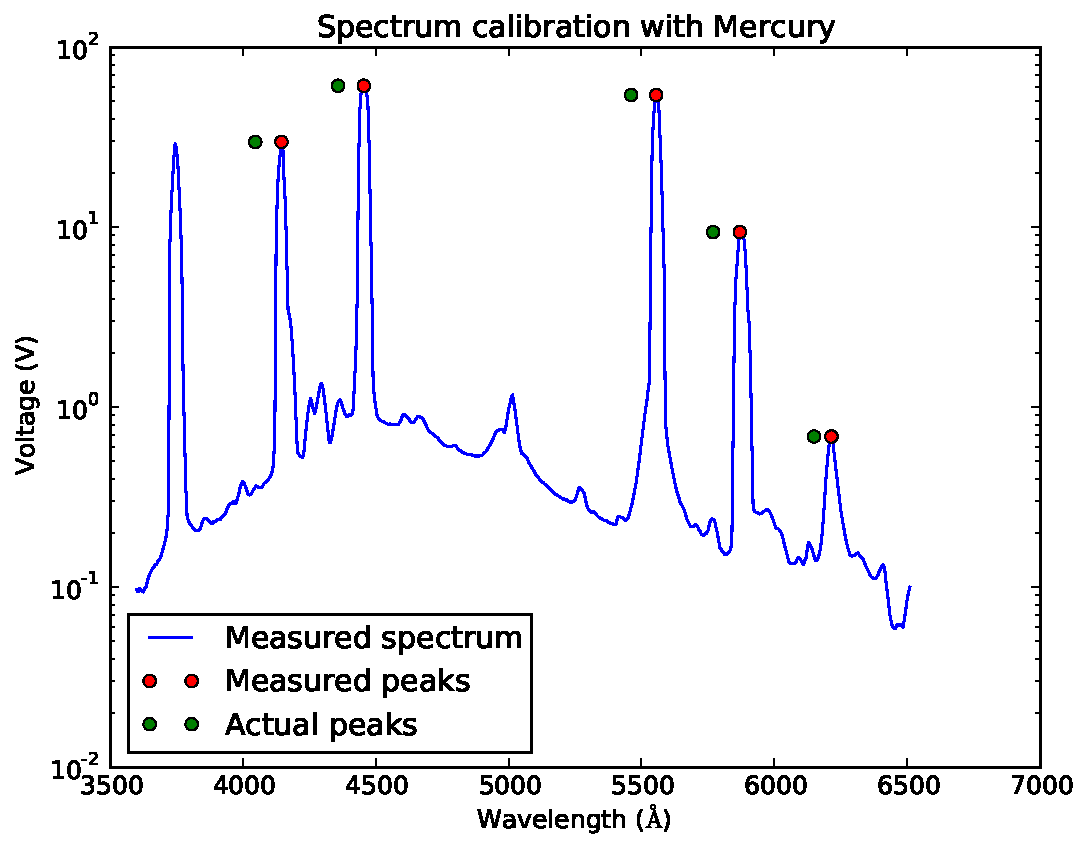
\includegraphics[width=\textwidth]{figures/merc_spec.pdf}
    \end{minipage}
    \hspace{0.5em}
    \begin{minipage}[t]{0.45\textwidth}
        \centering
        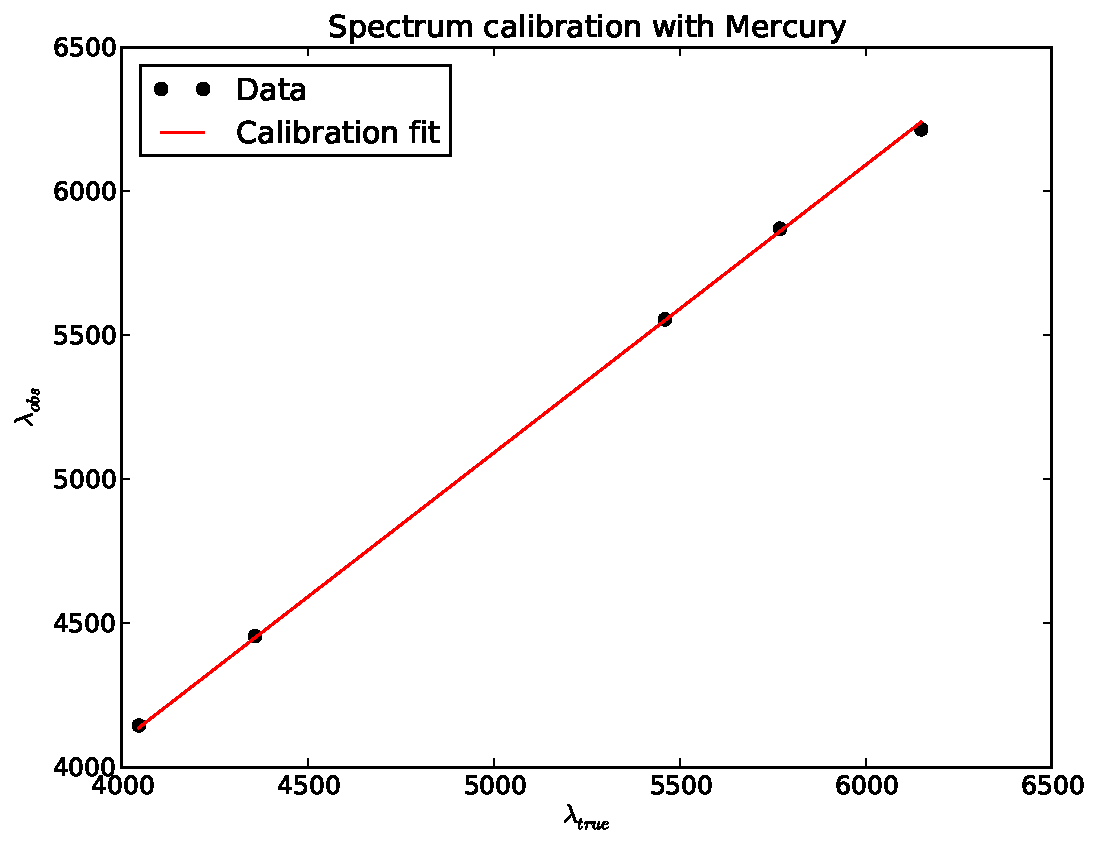
\includegraphics[width=\textwidth]{figures/merc_calib.pdf}
    \end{minipage}
    \caption{(left) Spectrum of mercury, plus a comparison of the observed peaks
    vs the average peaks illustrating the calibration that needed to be made.
    (right) Calibration plot relating the observed spectral lines of mercury to
    the accepted line values.}
    \label{mercury}
\end{figure}

Data collection is done by scanning through a range of wavelengths on the
spectrometer and recording the signal corresponding to each wavelength in
LabVIEW. This is pretty straightforward, but there are corrections that need to
be made to the wavelengths that the spectrometer claims versus actual wavelength
values. The calibration curve for this is done by measuring the spectrum of
mercury and correcting it using the accepted values of the emission lines for
mercury. Mercury's spectrum, plus the calibration curve used to correct the
wavelengths, can be seen in Figure~\ref{mercury}. The calibration curve is
fairly straightforward to add to the measured wavelengths and should give the
correct wavelengths.

\subsection{Analysis}

% Hydrogen spectrum and linear fit for finding Rydberg's constant.
\begin{figure}
    \centering
    \begin{minipage}[t]{0.45\textwidth}
        \centering
        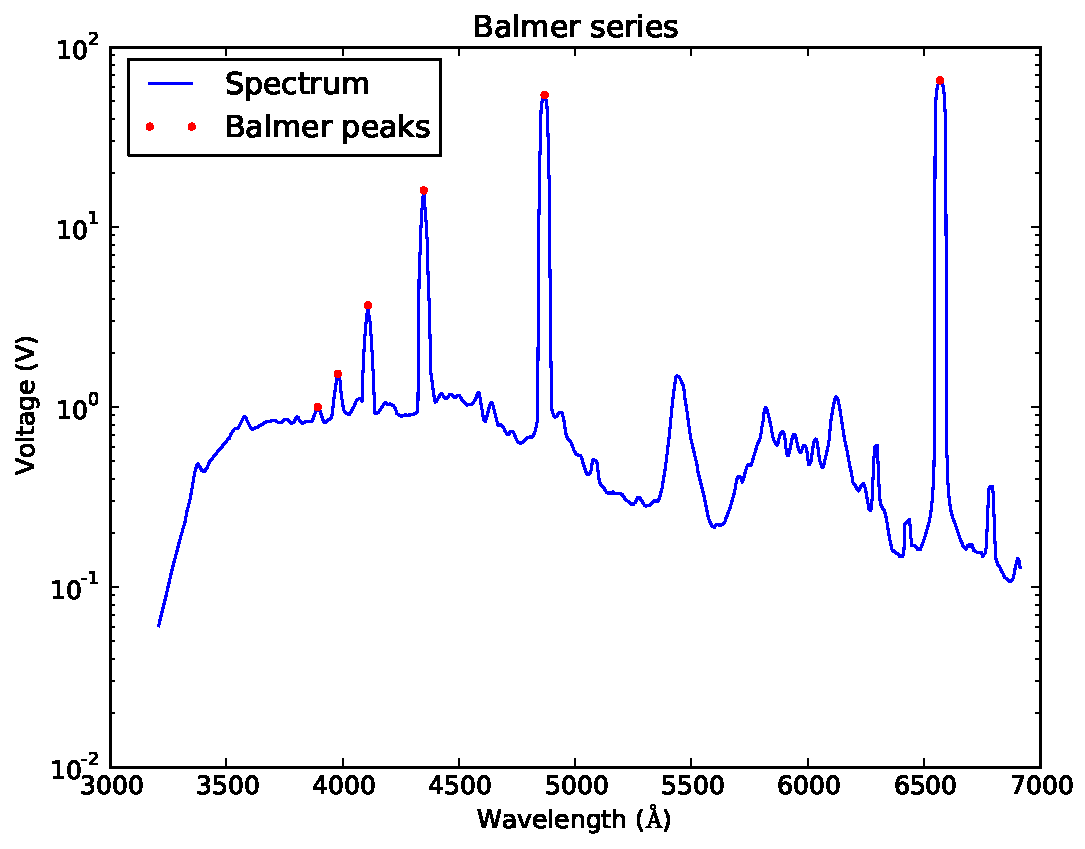
\includegraphics[width=\textwidth]{figures/hydrogen_spec.pdf}
    \end{minipage}
    \hspace{0.5em}
    \begin{minipage}[t]{0.45\textwidth}
        \centering
        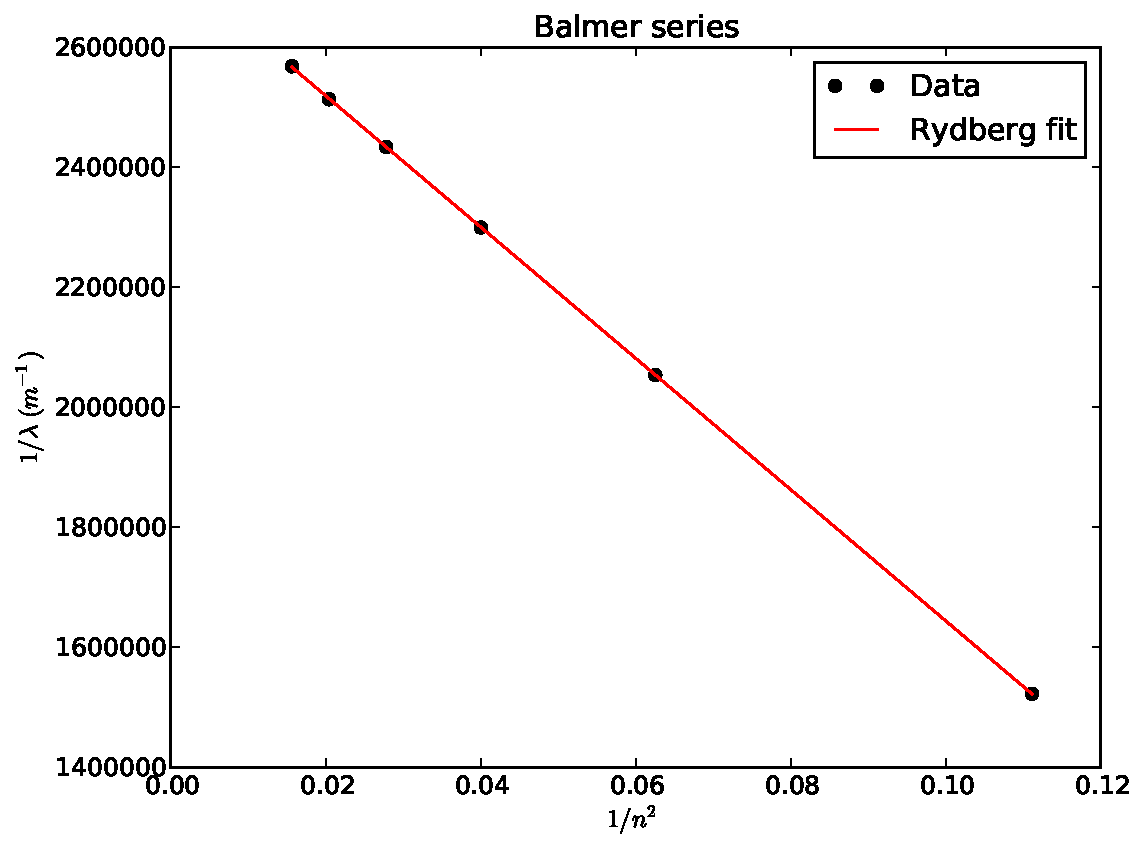
\includegraphics[width=\textwidth]{figures/rydberg.pdf}
    \end{minipage}
    \caption{(left) The spectrum of hydrogen for visible wavelengths. Note that
    the wavelengths peaks get closer and closer together when moving from left
    to right, like $1 / n^2$. (right) Linear fit between $1 / \lambda$ and 
    $1 / n^2$.}
    \label{hydrogen}
\end{figure}

Calculating the Rydberg constant from \eqref{rydberg} is fairly straightforward.
This is done first by correcting the measured wavelengths that LabVIEW records
using the calibration curve generated from the spectrum of mercury. Next, the
peaks in the spectrum are detected and mapped to the quantum number that
corresponds to the emission line. This can be done by noting that the distances
in wavelengths in Figure~\ref{hydrogen} seem to get smaller, maybe as $1/n^2$,
when moving from left to right. It can be seen from \eqref{rydberg}  and
Figure~\ref{hydrogen} that the inverse wavelength is linearly proportional to
$1 / n^2$. The fit can then be used to to calculate Rydberg's constant from both
the slope ($m = -R$) and the y-intercept ($b = R/4$). The weighted average of
the two measurements of $R$ can be taken to calculate a final value of $R$. \\

In order to compute the weighted average for any measurement of a specific
value, one must know the uncertainties on each term being used to compute the
average. This can be done by using the definition of $\chi^2$, and the
condition that the best fit yields a $\chi^2 / ndf = 1$. Assuming that the error
for all inverse wavelength is constant, it can easily be shown that
\begin{equation}
    \sigma^2 = \frac{1}{ndf} \sum_{i=0}^N \left(y_i - m x_i - b\right)^2
\end{equation}
This can be used to give the errors of the coefficients computed in the linear
fit which are \cite{LyonsError}
\begin{equation}
    \begin{array}{lcr}
        \sigma^2\left(m\right) & = & 
        \left(\dfrac{1}{\sigma^2}\sum x_i^2 \right)^{-1} \\
        \ \\
        \sigma^2\left(b\right) & = & \dfrac{\sigma^2}{N} + \langle x \rangle^2
            \sigma^2\left(m\right)
    \end{array}
    \label{coeferr}
\end{equation}
where $\langle x \rangle = \langle 1 / n^2 \rangle$ and $N$ is the number of
data points used in the least squares fit. Applying this to the two values of
$R$ gives a value of $R = 1.095 \times 10^7 \pm 2 \times 10^4\ m^{-1}$. This is
pretty close to the accepted value of the Rydberg constant, although it seems as
the error is way too small.

\section{Zeeman Splitting}

Zeeman splitting is the effect that occurs when electrons are placed in an
external magnetic field. What happens is that when the magnetic field is applied
to the electrons, the energy levels, which are degenerate, split and become
either non-degenerate or less degenerate. This experiment uses helium gas to
measure the Zeeman splitting, and the Hamiltonian for the electrons is
\begin{equation}
    \hat{H} = -\vec{\mu} \cdot \vec{B}_{ext}
\end{equation}
where $\vec{\mu}$ is the magnetic moment of the electron. Quantum mechanics
shows that the energy separation of the splitting is \cite{BransdenQM}
\begin{equation}
    \Delta E = m_J g_J \mu_B B_{ext}
\end{equation}
where $m_J$ is the quantum number describing the total momentum in the $\hat{z}$
direction, $g_J$ is the famous Lande-$g$ factor, and $\mu_B$ is the Bohr
magneton. The actual effect of Zeeman splitting is very small and it takes a
precision measurement in order to observe it. In this experiment, Zeeman
splitting of the red spectral line of helium was measured, and that corresponds
to a state change of $^1D \rightarrow ^1P$.

%Since the energy splitting
%corresponds to a frequency difference, which is related to a wavelength
%difference by \eqref{broadswitch}. Of course, using \eqref{broadswitch} is only
%valid because the splitting is tiny. From this, it can be seen that
%\begin{equation}
%    \frac{hc}{\lambda^2}\Delta \lambda = m_J g_J \mu_B B_{ext}
%\end{equation}
%where $\lambda$ is the splitting wavelength.

\subsection{Experimental Setup}

% Block diagram of the Zeeman splitting experiment
\begin{figure}
    \centering
    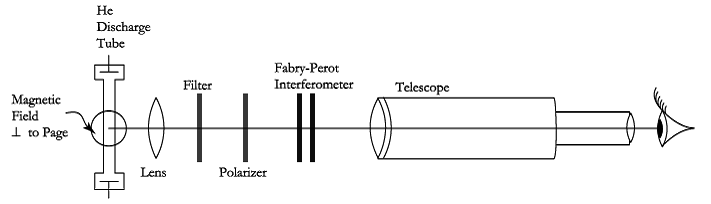
\includegraphics[width=\textwidth]{figures/Atm1image004.png}
    \caption{Block diagram of the Zeeman splitting experiment.}
    \label{zeeblock}
\end{figure}

A block diagram of the Zeeman splitting experiment can be seen in
Figure~\ref{zeeblock}. This experiment measures the Zeeman splitting by
observing ring shapes in an image. How it works is that a helium discharge tube
is placed inside of a pair of Helmholtz coils. Light emitted from the gas tube
gets focused through a red filter, which removes most of the spectral lines.
After the light goes through the filter, it passes through a polarizer, which
is set to only admit frequencies coming from energy level splittings of
$\Delta m_J = \pm 1$. The polarized light then passes through a Fabry-Perot
interferometer, which is used because it has a high wavelength resolving power.
After the light goes through the interferometer, it gets recorded by a CCD
camera and in the rare case that the camera software (or even Windows) on the
computer the camera is connected to is actually working properly, or at all, a
bitmap of the Zeeman rings can be taken and saved.

\subsection{The Fabry-Perot Interferometer}

The Fabry-Perot interferometer is what allows the Zeeman splitting to be
observed. A diagram demonstrating the basics of how it works can be seen in
Figure~\ref{fabryperot}. The interferometer is made of two partially reflecting
mirrors and a lens. How the interferometer works is that an incoming beam of
light enters the interferometer, and then gets reflected off on the second
mirror. Part of the light beam goes through the mirror and another part gets
reflected back to the first mirror, which then reflects another ray of light at
the second mirror at the same angle of incidence as the original beam. All of
the beams that were generated from the original beam and the mirror sequence
then pass through the lens in the interferometer, which is designed to focus the
beams at infinity. The beams that come out of the lens produce and intensity
distribution of \cite{LabManual}
\begin{equation}
    I\left(\theta, t\right) = 
    \frac{I_0}{1 + \dfrac{4R}{\left(1-R\right)^2}\sin^2 \dfrac{\delta}{2}}
\end{equation}
where $\delta = 2\pi \frac{2t\cos\theta}{\lambda}$, $t$ is the spacing of the
interferometer, and $R$ is the reflectance of the mirrors in the interferometer.
The smallest difference in wavenumber that can be resolved, which corresponds to
the smallest energy difference that can be resolved, is \cite{LabManual}
\begin{equation}
    \delta \sigma = \frac{1}{2tN_R}
\end{equation}
and 
\begin{equation}
    N_R = \pi \frac{\sqrt{R}}{1-R}
\end{equation}

For the interferometer used in the experiment, $t$ is $8.1\ mm$ and $R$ is 0.90,
so $N_R = 29.8$ and $\delta\sigma = 2.07\ m^{-1}$.

% Schematic diagram of the Fabry-Perot interferometer
\begin{figure}
    \centering
    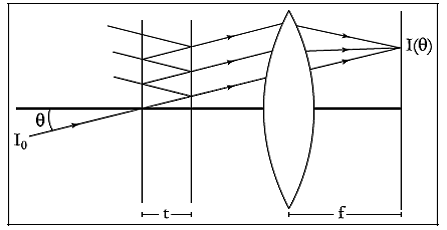
\includegraphics[width=0.6\textwidth]{figures/Atm1image005.png}
    \caption{Schematic diagram of the workings of the Fabry-Perot
    interferometer.}
    \label{fabryperot}
\end{figure}

\subsection{Zeeman Rings}

An example of data from this experiment can be seen in Figure~\ref{nofield}. In
that case, there is no magnetic field being applied to the helium gas. When a
magnetic field does get applied to the helium, the rings start to split. There
are two splittings of interest in this experiment, which can be seen in
Figure~\ref{zeefield}. The exact procedure for using these images to calculate
the Bohr magneton shall be described in the next section. However, it should be
noted that originally, a calibration curve to map the voltage applied to the
Helmholtz coils to the magnetic field produced by the coils was made. However,
since there were only two Zeeman splittings of interest for the final analysis,
directly measuring the magnetic field for those two splittings seemed to be
simpler.

\subsection{The Bohr Magneton}

The Zeeman splitting experiment can be used to get a measurement of the Bohr
magneton $\mu_B$. The energy difference between the split levels is
$\Delta E = hc \Delta \nu$. In this experiment, the value of $\Delta \nu$ is
known to be \cite{ExpModern}
\begin{equation}
    \Delta \nu = \frac{\Delta n}{2t}
\end{equation}
where $\Delta n$ is the fractional difference in the splitting of the Zeeman
rings and $t$ is the spacing of the Fabry-Perot interferometer. Setting the
energy difference equal to the splitting energy difference gives
\begin{equation}
    \frac{hc\Delta n}{2t} = \mu_B B_{ext}
\end{equation}
where $m_J$ and $g_J$ are both equal to one. This gives an expression for the
Bohr magneton that relates to the quantities measurable in the experiment as
\begin{equation}
    \mu_B = \frac{hc\Delta n}{2tB_{ext}}
    \label{bohr_ub}
\end{equation}

The main uncertainty that comes into \eqref{bohr_ub} is from uncertainty in the
magnetic field, and this is assuming that any uncertainty in the Fabry-Perot
thickness is negligible. Since the variance of the Bohr magneton and the
external magnetic field are related as
$\sigma^2_\mu / \mu^2 = \sigma^2_B / B^2$, it can easily be demonstrated that
\begin{equation}
    \sigma_{\mu_B} = \frac{hc\Delta n}{2tB^2_{ext}} \sigma_B
\end{equation}

Figure~\ref{zeefield} shows the two Zeeman splittings of interest. The magnetic
fields measured for these fields were $B_{ext} = 0.278\ T$ when $\Delta n = 1/3$
and $B_{ext} = 0.410\ T$ when $\Delta n = 1/2$. In both cases, the uncertainty
of the field is about $0.005\ T$. These values of the magnetic fields give
measurements of the Bohr magneton of $\mu_B = 1.47\times 10^{-23}\ J/T$ and 
$\mu_B = 1.50\times 10^{-23}\ J/T$. These values, along with their
uncertainties, give a weighted average of $\mu_B = 1.49\times 10^{-23} \pm
2\times 10^{-25}\ J/T$. This is on the right order of magnitude of the Bohr
magneton, but both measured values are off by a scaling factor, which seems
constant. The magnetic field detector used in the experiment was checked against
a source of known value and seemed to be working properly. It's possible that
there could be an error in the value given for $t$, but the range of $t$ is
small, so that wouldn't explain everything.

% Zeeman splitting figures.
\begin{figure}
    \centering
    \begin{minipage}[t]{0.45\textwidth}
        \centering
        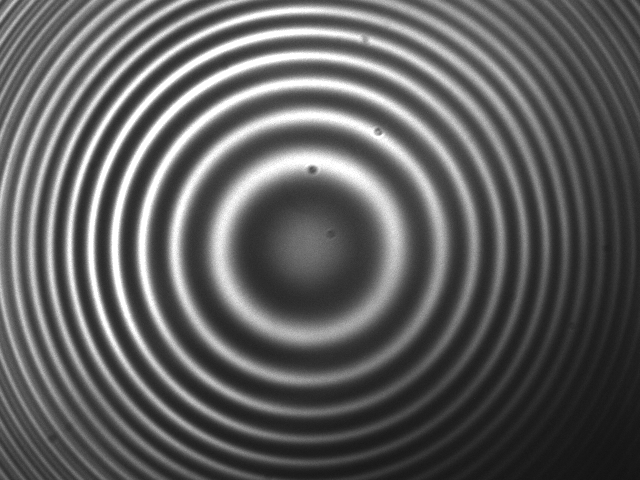
\includegraphics[width=\textwidth]{figures/0V.png}
    \end{minipage}
    \hspace{0.5em}
    \begin{minipage}[t]{0.45\textwidth}
        \centering
        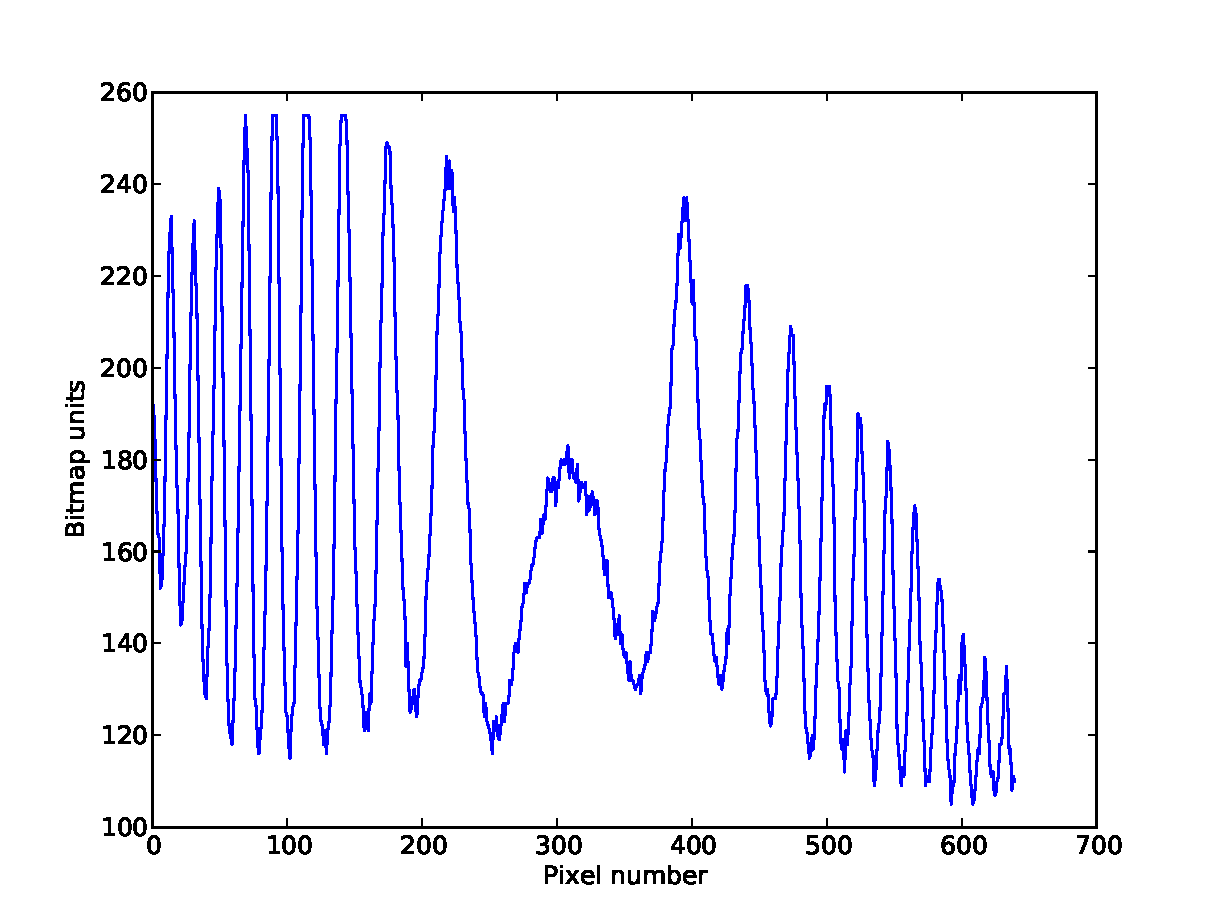
\includegraphics[width=\textwidth]{figures/zeeman_center.pdf}
    \end{minipage}
    \caption{(left) Bitmap of the Zeeman rings. (right) The center row of the
    left image. No magnetic field is currently being applied to the helium.}
    \label{nofield}
\end{figure}

\newpage

\begin{figure}
    \centering
    \begin{minipage}[t]{0.45\textwidth}
        \centering
        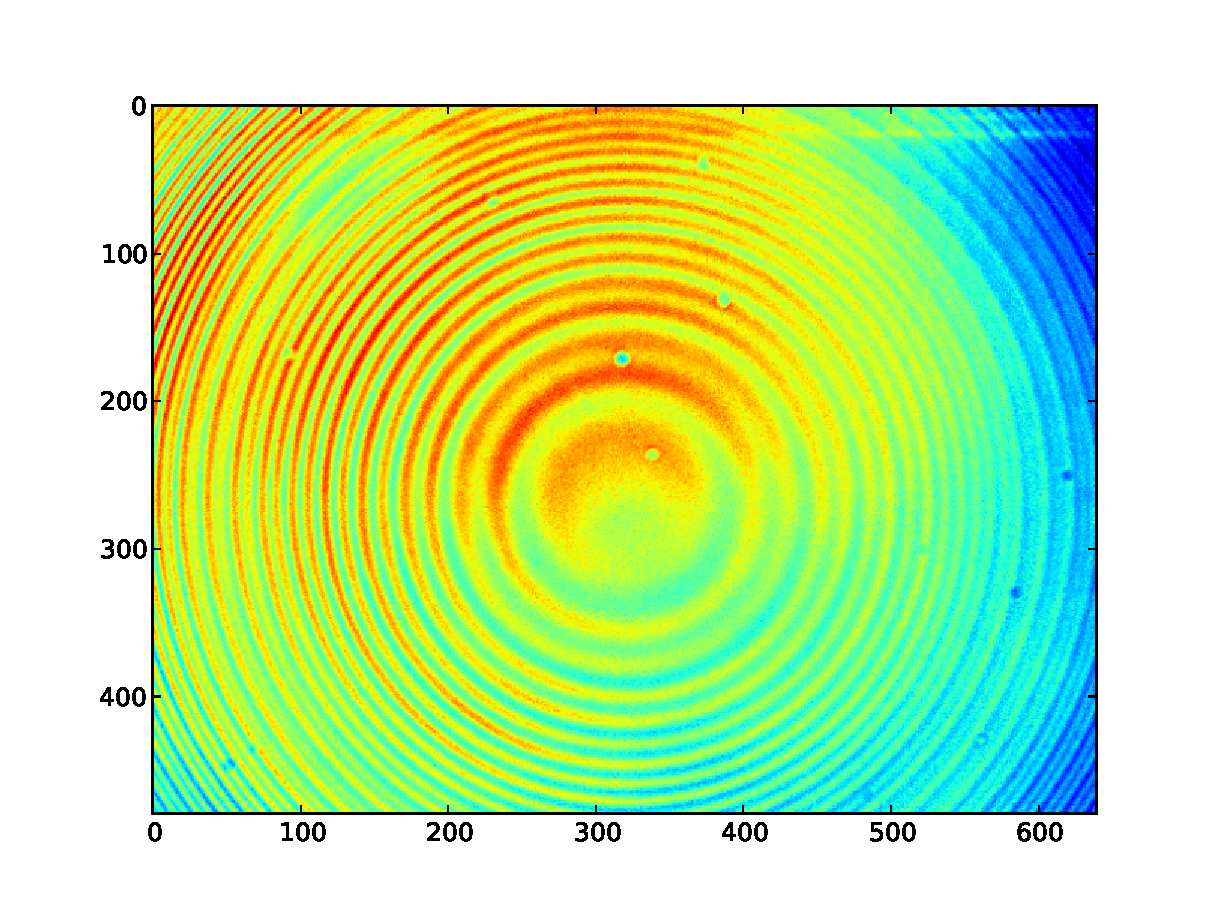
\includegraphics[width=\textwidth]{figures/Small9V_col.pdf}
    \end{minipage}
    \hspace{0.5em}
    \begin{minipage}[t]{0.45\textwidth}
        \centering
        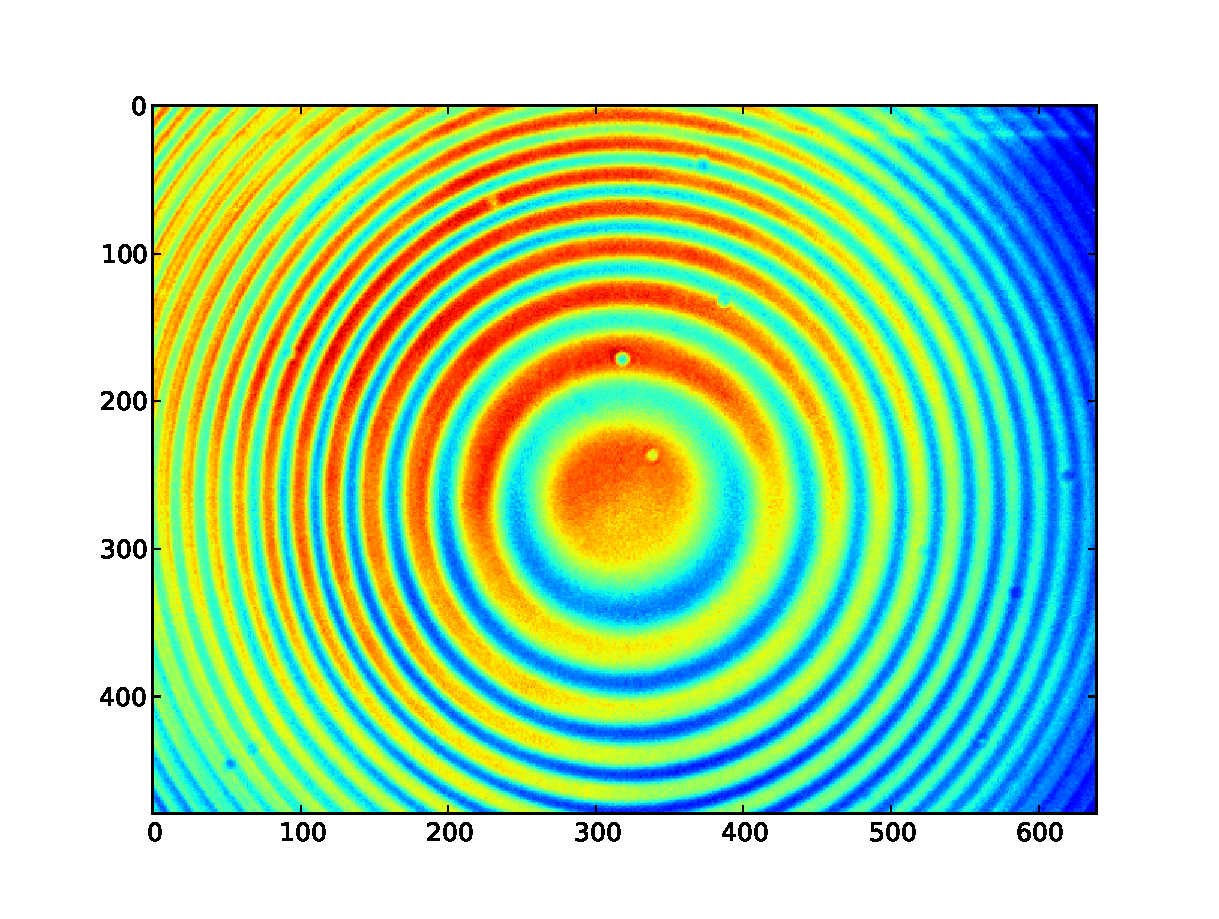
\includegraphics[width=\textwidth]{figures/Small15V_col.pdf}
    \end{minipage}
    \caption{(left) Evenly spaced rings from the splitting corresponds to a
        $\Delta n = 1/3$.
    (right) Overlapping rings from the splitting corresponds to
    $\Delta n = 1/2$. Both images have been colorized to make the splitting more
    clear looking.}
    \label{zeefield}
\end{figure}

\bibliographystyle{unsrt}
\bibliography{reference_list}{}

\newpage

\begin{figure}
    \centering
    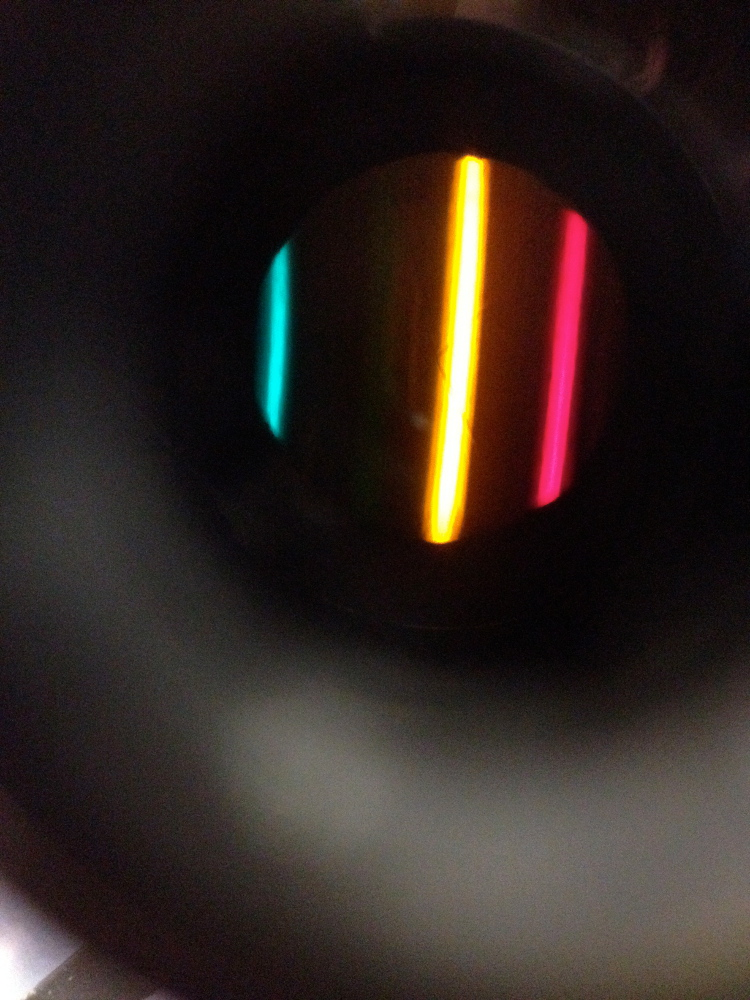
\includegraphics[width=\textwidth]{figures/IMG_1309.jpg}
    \caption{Some of the spectral lines of helium viewed from the prism
    monochromator.}
\end{figure}

\end{document}  
